
\documentclass{beamer}
\usecolortheme{dove}
\setbeamertemplate{navigation symbols}{}
\usepackage{amsmath,amssymb,amsfonts,amsthm, multicol, subfigure, color}
\usepackage{bm}
\usepackage{graphicx}
\usepackage{tabularx}
\usepackage{booktabs}
\usepackage{hyperref}
\usepackage{pdfpages}
\usepackage{xcolor}
\definecolor{seagreen}{RGB}{46, 139, 87}
\definecolor{mustard}{RGB}{234, 170, 0}
\def\independenT#1#2{\mathrel{\rlap{$#1#2$}\mkern2mu{#1#2}}}
\newcommand\indep{\protect\mathpalette{\protect\independenT}{\perp}}
\def\log{\text{log}}
\newcommand\logit{\text{logit}}
\newcommand\iid{\stackrel{\text{iid}}{\sim}}
\newcommand\E{\text{E}}
\newcommand\V{\text{V}}
\renewcommand\P{\text{P}}
\newcommand{\Cov}{\text{Cov}}
\newcommand{\Cor}{\text{Cor}}
\newcommand\doop{\texttt{do}}
\usepackage{stackrel}
\usepackage{tikz}
\usetikzlibrary{arrows,shapes.arrows,positioning,shapes,patterns,calc}
\newcommand\slideref[1]{\vskip .1cm \tiny \textcolor{gray}{{#1}}}
\newcommand\red[1]{\color{red}#1}
\newcommand\blue[1]{\color{blue}#1}
\newcommand\gray[1]{\color{gray}#1}
\newcommand\seagreen[1]{\color{seagreen}#1}
\newcommand\purple[1]{\color{purple}#1}
\newcommand\orange[1]{\color{orange}#1}
\newcommand\black[1]{\color{black}#1}
\newcommand\white[1]{\color{white}#1}
\newcommand\teal[1]{\color{teal}#1}
\newcommand\magenta[1]{\color{magenta}#1}
\newcommand\Fuchsia[1]{\color{Fuchsia}#1}
\newcommand\BlueGreen[1]{\color{BlueGreen}#1}
\newcommand\bblue[1]{\textcolor{blue}{\textbf{#1}}}
\newcommand\bred[1]{\textcolor{red}{\textbf{#1}}}
\newcommand\bgray[1]{\textcolor{gray}{\textbf{#1}}}
\newcommand\bgreen[1]{\textcolor{seagreen}{\textbf{#1}}}
\newcommand\bref[2]{\href{#1}{\color{blue}{#2}}}
\colorlet{lightgray}{gray!40}
\pgfdeclarelayer{bg}    % declare background layer for tikz
\pgfsetlayers{bg,main} % order layers for tikz
\newcommand\mycite[1]{\begin{scriptsize}\textcolor{darkgray}{(#1)}\end{scriptsize}}
\newcommand{\tcframe}{\frame{
%\small{
\only<1|handout:0>{\tableofcontents}
\only<2|handout:1>{\tableofcontents[currentsubsection]}}
%}
}

\newcommand{\goalsframe}{\begin{frame}{Learning goals for today}
By the end of class, you will be able to
\begin{itemize}
\item Estimate causal effects parametrically with OLS
\end{itemize} \vskip .2in
\end{frame}}

\usepackage[round]{natbib}
\bibliographystyle{humannat-mod}
\setbeamertemplate{enumerate items}[default]
\usepackage{mathtools}

\title{Studying Social Inequality with Data Science}
\author{Ian Lundberg}
\date{\today}

\begin{document}

\begin{frame}
\begin{tikzpicture}[x = \textwidth, y = \textheight]
\node at (0,0) {};
\node at (1,1) {};
\node[anchor = north west, align = left, font = \huge] at (0,.9) {Studying\\Social Inequality\\with Data Science};
\node[anchor = north east, align = right] (number) at (1,.9) {INFO 3370 / 5371\\Spring 2023};
\node[anchor = north, font = \Large, align = left] at (.5,.5) {\bblue{Causal Estimators}:\\Parametric estimation with OLS};
\end{tikzpicture}
\end{frame}

\goalsframe

\begin{frame}{Data}
We will examine the effect of education on log income\\using the data from the \bref{https://info3370.github.io/lessonplans/7b/}{PSID Prediction Challenge} \vskip .2in
Assume this causal DAG:
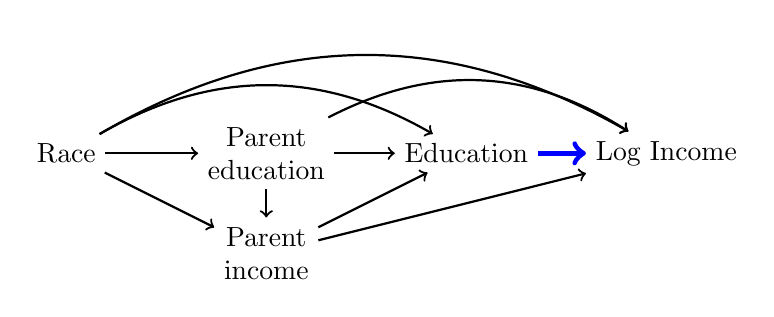
\begin{tikzpicture}[x = 1in, y = .5in]
\node (a) at (0,0) {Education};
\node (y) at (1,0) {Log Income};
\node[black] (x1) at (-2,0) {Race};
\node[align = center] (x2) at (-1,0) {Parent\\education};
\node[align = center, black] (x3) at (-1,-1) {Parent\\income};
\draw[->, line width = 2pt, black, blue] (a) -- (y);
\draw[->, thick, black] (x1) to[bend left] (a);
\draw[->, thick, black] (x1) to[bend left] (y);
\draw[->, thick, black] (x1) -- (x2);
\draw[->, thick, black] (x1) -- (x3);
\draw[->, thick, black] (x2) -- (x3);
\draw[->, thick, black] (x3) -- (a);
\draw[->, thick, black] (x3) -- (y);
\draw[->, thick] (x2) -- (a);
\draw[->, thick] (x2) to[bend left] (y);
\end{tikzpicture} \\
Ultimately, we will adjust for race, parent education, and parent income
\end{frame}

\begin{frame}{Model-based adjustment}
\begin{enumerate}
\item fit a model to predict the outcome
\item create two new data frames
\begin{itemize}
\item with education set to \texttt{college}
\item with education set to \texttt{high school}
\end{itemize} 
\item predict the outcome under each treatment
\item difference
\item average over all the people
\end{enumerate}

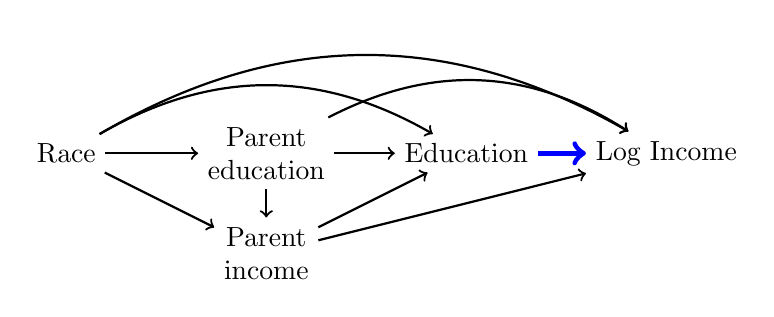
\begin{tikzpicture}[x = 1in, y = .5in]
\node (a) at (0,0) {Education};
\node (y) at (1,0) {Log Income};
\node[black] (x1) at (-2,0) {Race};
\node[align = center] (x2) at (-1,0) {Parent\\education};
\node[align = center, black] (x3) at (-1,-1) {Parent\\income};
\draw[->, line width = 2pt, black, blue] (a) -- (y);
\draw[->, thick, black] (x1) to[bend left] (a);
\draw[->, thick, black] (x1) to[bend left] (y);
\draw[->, thick, black] (x1) -- (x2);
\draw[->, thick, black] (x1) -- (x3);
\draw[->, thick, black] (x2) -- (x3);
\draw[->, thick, black] (x3) -- (a);
\draw[->, thick, black] (x3) -- (y);
\draw[->, thick] (x2) -- (a);
\draw[->, thick] (x2) to[bend left] (y);
\end{tikzpicture}
\end{frame}

\goalsframe


\end{document}

